\documentclass[a4paper,10pt]{article}

\usepackage[utf8]{inputenc}
\usepackage[T1]{fontenc}
\usepackage[margin=1cm]{geometry}
\usepackage{hyperref}
\usepackage{xcolor}
\usepackage{tabularx}
\usepackage{fontawesome5}
\usepackage{lastpage}
\usepackage{multicol}
\usepackage{graphicx}
\usepackage{libertinus}
\usepackage{parskip}
\usepackage[normalem]{ulem}
\usepackage{ragged2e}
\usepackage{enumitem}
\usepackage{avant}
\usepackage{pgfplots}
\usepackage{tikz}
\pgfplotsset{compat=1.18}

% Define colors based on the dayfox theme
\definecolor{background}{HTML}{f6f2ee}
\definecolor{foreground}{HTML}{3d2b5a}
\definecolor{brightforeground}{HTML}{643f61}
\definecolor{red}{HTML}{754E27}
\definecolor{darkblue}{HTML}{274A75}
\definecolor{blue}{HTML}{4F8DA0}
\definecolor{yellow}{HTML}{ac5402}
\definecolor{magenta}{HTML}{6e33ce}
\definecolor{cyan}{HTML}{287980}
\definecolor{white}{HTML}{f2e9e1}
\definecolor{leadershipbg}{HTML}{ECE9E5}
\definecolor{webdevbg}{HTML}{CAC7C4}

% Define the title
\newcommand{\doctitle}{Andres Monge - CV - English}

% Set the document title
\title{\doctitle}

\hypersetup{
    pdftitle={\doctitle},
    pdfauthor={Andres Monge},
    pdfsubject={CV},
    colorlinks=true,
    linkcolor=blue,
    filecolor=magenta,
    urlcolor=cyan,
}

\pagecolor{background}
\color{foreground}

\setlength{\parskip}{1em}

\newcommand{\skillstar}[1]{%
    \textcolor{darkblue}{%
        \ifnum#1>0$\bullet$\else$\circ$\fi%
        \ifnum#1>1$\bullet$\else$\circ$\fi%
        \ifnum#1>2$\bullet$\else$\circ$\fi%
        \ifnum#1>3$\bullet$\else$\circ$\fi%
        \ifnum#1>4$\bullet$\else$\circ$\fi%
    }%
}

% New command for full-width colorbox with original text margins
\newcommand{\fullwidthcolorbox}[2]{%
  \noindent\makebox[\linewidth]{%
    \colorbox{#1}{%
      \parbox{\dimexpr\paperwidth-2\fboxsep\relax}{%
        \hspace{\dimexpr\oddsidemargin+1in}%
        \begin{minipage}{\textwidth}
        #2
        \end{minipage}%
        \hspace{\dimexpr\evensidemargin+1in}%
      }%
    }%
  }%
}

\begin{document}

\noindent
\begin{minipage}[t]{0.7\textwidth}
{\Large\bfseries\fontfamily{pag}\selectfont Andres Monge - Python Technical Lead}
\end{minipage}%
\begin{minipage}[t]{0.23\textwidth}
\raggedleft
\begin{tabularx}{\linewidth}{XXXX}
    \href{https://www.linkedin.com/in/aemonge/}{\faLinkedin} &
    \href{https://github.com/aemonge}{\faGithub} &
    \href{https://stackoverflow.com/users/1360897/aemonge}{\faStackOverflow} &
    \href{https://pypi.org/user/aemonge/}{\faPython} \\
\end{tabularx}
\end{minipage}

\vspace{0.5cm}

\noindent
\begin{minipage}[t]{0.65\textwidth}
\begin{minipage}[t]{\dimexpr\linewidth-25px}
\justifying

I am a \textbf{seasoned technical lead and solutions architect} with a passion for \textbf{Python development, machine learning, and MLOps}. I am a \textbf{hands-on leader} who thrives on solving complex problems and delivering value. My leadership style is rooted in \textbf{technical excellence, empathy, and a coach-mentor approach}.

\vspace{0.5cm}

I am seeking a \textbf{Python Tech Lead role} where I can apply these qualities to create impactful solutions. With \textbf{over 15 years of experience}, I have demonstrated that my architectural design skills are transferable across various languages.

    \section*{\large SHIFTING TO PYTHON AND AI}
    \textbf{\textit{Python Technical Lead}}
    \textit{\small Origen, Madrid, Spain (2024) (presently)}
    \vspace{0.3cm}
    \begin{itemize}[leftmargin=*]
        \item \textbf{Responsibilities:} Led the team with strict adherence to high-quality code guidelines, ensuring maintainable and scalable solutions; mentored and guided two peers, fostering a collaborative environment and driving team performance.
        \item \textbf{Accomplishments:} Successfully created an ad-hoc data management solution, resulting in a monthly cost savings of \$2,000; fully refactored the platform from a non-maintainable state to a PEP8 compliant, well-documented, and guideline-driven architecture.
        \item \textbf{Technologies:} Python, Kubernetes, Bash, SQL, Docker, Numpy, Pandas.
        \item \textbf{Personal Growth:} Gained deeper insights into AI team workflows, understanding their expectations and limitations; developed effective communication skills to provide solutions that enhance their performance; refined my ability to lead AI and Machine Learning teams, bridging my managerial background with technical expertise in AI development.
    \end{itemize}

    \vspace{0.5cm}

    \textbf{\textit{Python Technical Lead}}
    \textit{\small Babiopower, California, USA (remote) (2023-2024) (freelance)}
    \vspace{0.3cm}
    \begin{itemize}[leftmargin=*]
        \item \textbf{Responsibilities:} Built the company software to generate a solar panels installation proposal;
    Managed the team to build the front-end application and help in the back-end.
        \item \textbf{Accomplishments:} Built the entirety of the system using Python, MongoDB, and Docker images;
    Mentored and guided two more developers.
        \item \textbf{Technologies:} Python, FastAPI, Pydantic, MongoDB, Docker.
        \item \textbf{Personal Growth:} Deepened expertise in Python and FastAPI, gained valuable experience in machine ops AI.
    \end{itemize}

    \vspace{0.5cm}

    \textbf{\textit{Machine Learning Engineer}}
    \textit{\small Delorean group, Mexico city (remote) (2023) (freelance)}
    \vspace{0.3cm}
    \begin{itemize}[leftmargin=*]
        \item \textbf{Responsibilities:} Built a Convolutional Neural Network (CNN) that identified landmarks for a small
    tourism company.
        \item \textbf{Accomplishments:} Developed a CNN model that accurately identified and classified various
    landmarks, enhancing the company's tourism offerings and customer engagement.
        \item \textbf{Technologies:} Python, PyTorch, and Transformers.
        \item \textbf{Personal Growth:} Applied Python and AI skills in a real-world context, deepened expertise in these
    areas, and demonstrated the practical value of AI in enhancing business operations.
    \end{itemize}

    \vspace{0.5cm}

    \textbf{\textit{Front-end Team Lead}}
    \textit{\small Bonial / Kaufda.be, Berlin, Germany (2017)}
    \vspace{0.3cm}
    \begin{itemize}[leftmargin=*]
        \item \textbf{Responsibilities:} Developed Micro-fronts using Polymer for the UI of an AI training system; Created
    an infinite undo/redo global interface and a hyper-fast UI tag autocomplete using local storage for
    optimization.
        \item \textbf{Accomplishments:} Developed a tag component that was incredibly fast by using a double cache
    system; Created a grid splitter directly into the AI tool, which accelerated the selection of sections by
    300x.
        \item \textbf{Technologies:} Polymer, AI.
        \item \textbf{Personal Growth:} Gained valuable experience in AI and developed proficiency in Polymer.
    \end{itemize}
\end{minipage}\hspace{5px}
\end{minipage}%
\begin{minipage}[t]{0.33\textwidth}
    \vspace{-.3cm}

    \centering
    \fbox{
\includegraphics[width=0.8\linewidth]{avatar.png}}

    \vspace{0.5cm}
    \justifying
    \textbf{"Empowering teams to build innovative solutions with a focus on value and efficiency."}

\vspace{0.5cm}
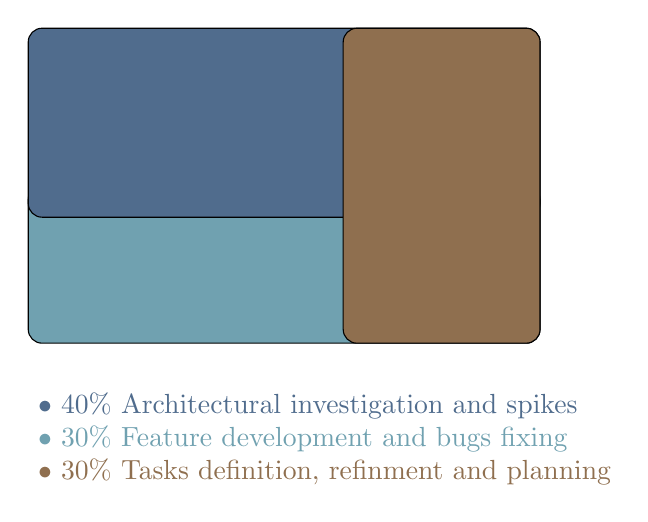
\begin{tikzpicture}
% Define the rectangles with rounded corners
\draw[fill=blue!80!background, rounded corners=5pt] (0,0) rectangle (6.5,2);
\draw[fill=darkblue!80!background, rounded corners=5pt] (0,1.6) rectangle (6.5,4);
\draw[fill=red!80!background, rounded corners=5pt] (4,0) rectangle (6.5,4);

% Add explanations below the squares as bullet points
\node[anchor=north west, align=left] at (0, -0.5) {
    \textcolor{darkblue!80!background}{$\bullet$ 40\% Architectural investigation and spikes}\\
    \textcolor{blue!80!background}{$\bullet$ 30\% Feature development and bugs fixing}\\
    \textcolor{red!80!background}{$\bullet$ 30\% Tasks definition, refinment and planning}
};
\end{tikzpicture}

\vspace{0.1cm}
\section*{\large Software Languages}
\begin{tabularx}{\linewidth}{cXr}
    \faPython & Python & \skillstar{4} \\
    \faDocker & DevOps & \skillstar{3} \\
    \faDatabase & Databases & \skillstar{4} \\
    \faTerminal & Bash & \skillstar{4} \\
    \faGem & pytorch & \skillstar{2} \\
    \faGem & numpy & \skillstar{2} \\
    \faJs & JavaScript & \skillstar{4} \\
    \faCss3 & CSS/HTML & \skillstar{4} \\
\end{tabularx}

    \vspace{0.5cm}
    \section*{\large Spoken Languages}
    \begin{tabular}{cl}
        \faLanguage & Spanish (Mother Tongue) \\
        \faLanguage & English (Bilingual - C1) \\
    \end{tabular}
\end{minipage}

\newpage

\fullwidthcolorbox{leadershipbg}{%
\vspace{0.3cm}

\section*{\large LEADERSHIP - TECH LEAD AND MANAGER}
\textbf{\textit{Senior Engineering Manager}}
\textit{\small Lavanda, united kingdom (remote) (2022 - 2023)}
\vspace{0.3cm}
\begin{itemize}[leftmargin=*]
    \item \textbf{Responsibilities:} Served as a line manager for two squads; Coordinated with the CTO and CPO to
    design and develop features to alleviate customer churn.
    \item \textbf{Accomplishments:} Managed a team of 10 software engineers; Created an efficient algorithm to
    allocate randomized bookings with range and date constraints.
    \item \textbf{Technologies:} Python / Ruby on Rails.
    \item \textbf{Personal Growth:} Enhanced skills in managing a team and developed proficiency in Python and Ruby
    on Rails.
\end{itemize}
\vspace{0.5cm}

\textbf{\textit{Senior Engineering Manager}}
\textit{\small Global Savings Group, Germany (remote) (2021 - 2022)}
\vspace{0.3cm}
\begin{itemize}[leftmargin=*]
    \item \textbf{Responsibilities:} Managed a team of 7 software engineers; Kept the legacy code and systems active
    and clean of critical bugs, while participating in the discovery and planning of a company-wide code
    refactoring.
    \item \textbf{Accomplishments:} Designed and developed a web-crawler that saved the company 500€ weekly costs.
    \item \textbf{Technologies:} JavaScript, Python, HTML, (TS) React.
    \item \textbf{Personal Growth:} Gained valuable experience in remote management and developed proficiency in
    solutions architecture.
\end{itemize}
\vspace{0.5cm}

\textbf{\textit{Technical Lead / Software Architect}}
\textit{\small GFT / Santander Global Tech, Madrid, Spain (2018 - 2021)}
\vspace{0.3cm}
\begin{itemize}[leftmargin=*]
    \item \textbf{Responsibilities:} Served as a technical coordinator and solutions architect for development teams;
    Investigated new technologies and methodologies to accelerate delivery times and increase overall
    quality.
    \item \textbf{Accomplishments:} Designed a solution to generate documentation and dependency hierarchy
    automatically; Proved increase of 120% in delivery time in two projects designing ATDD; Became the
    go-to person for any DevOps and pipeline enhancement in the project, and led two USA teams to
    perform twice as better by creating better tools and guiding the team into knowing and using such
    tools.
    \item \textbf{Technologies:} Angular, JavaScript, Python scripting, bash, UML-Diagrams.
    \item \textbf{Personal Growth:} Enhanced my skills in team coordination and solutions architecture.
\end{itemize}
\vspace{0.5cm}
}% End of previous \fullwidthcolorbox
\begin{samepage}
\vspace{-1cm}% Adjust this value as needed
\fullwidthcolorbox{background}{%
\vspace{0.5cm}
\section*{\large WEB DEVELOPER}

\textbf{\textit{Team Lead / Developer}}
\textit{\small S|NGULAR / BBVA, Madrid, Spain (2013 - 2017)}
\vspace{0.3cm}
\begin{itemize}[leftmargin=*]
    \item \textbf{Responsibilities:} Mentored developers to implement modules and components, instead of jQuery; Participated in the construction of
    the CD/CI with GULP and git-flow; Developed an Angular component hosting a ReactJS module.
    \item \textbf{Accomplishments:} Successfully developed an Angular component hosting a ReactJS module.
    \item \textbf{Technologies:} Angular, ReactJS, jQuery, GULP, git-flow.
    \item \textbf{Personal Growth:} Enhanced my skills in mentoring and leading a team, and developed proficiency in Angular and ReactJS.
\end{itemize}

\vspace{0.5cm}

\textbf{\textit{Developer / Architect}}
\textit{\small Adesis (GFT), Madrid, Spain (2012 - 2013)}
\vspace{0.3cm}
\begin{itemize}[leftmargin=*]
    \item \textbf{Responsibilities:} Led the creation of robust software for the insurance sector, developing architectural components using front-end
    skills and leading with backend skills; Developed a personal finance manager app using AngularJS and led a NodeJS (Sails) developer.
    \item \textbf{Accomplishments:} Successfully developed a personal finance manager app and led a NodeJS developer.
    \item \textbf{Technologies:} AngularJS, NodeJS (Sails).
    \item \textbf{Personal Growth:} Gained valuable experience in front-end architecture and developed proficiency in AngularJS and NodeJS.
\end{itemize}

\vspace{0.5cm}

\textbf{\textit{Developer}}
\textit{\small C.B.I., Madrid, Spain (2010 - 2012)}
\vspace{0.3cm}
\begin{itemize}[leftmargin=*]
    \item \textbf{Responsibilities:} Developed end-to-end modules using BackboneJS and PHP for an ad-hoc SAP-like system.
    \item \textbf{Accomplishments:} Created a unique plugin for data import/export from XLS into SQL, parsing the data according to the system
    architecture and schemas.
    \item \textbf{Technologies:} BackboneJS, PHP, WordPress.
    \item \textbf{Personal Growth:} Enhanced my skills in client interaction and project management.
\end{itemize}

\vspace{0.5cm}

\textbf{\textit{Freelance Developer}}
\textit{\small Madrid, Spain (2008 - 2013)}
\vspace{0.3cm}
\begin{itemize}[leftmargin=*]
    \item \textbf{Responsibilities:} Developed custom websites for international clients using open-source back-end frameworks and vanilla front-
    ends; Created ad-hoc themes and plugins to provide tailored tools for clients.
    \item \textbf{Accomplishments:} Successfully delivered multiple websites including Universidad Rey Juan Carlos.
    \item \textbf{Technologies:} Joomla, WordPress, Drupal, OsCommerce, PHP.
    \item \textbf{Personal Growth:} Gained valuable experience in client interaction and developed proficiency in various CMS and e-commerce
    platforms.
\end{itemize}

\vspace{0.5cm}
}

\end{samepage}  % Add this line to close the samepage environment

\end{document}
